\documentclass{beamer}
\title{Building Recommender Systems}
\subtitle{Lecture 8}
\author{Boris Shminke}
\institute{Université Côte d'Azur, CNRS, LJAD, France}
\date{14/01/2021}
\AtBeginSection[]{
  \begin{frame}
    \frametitle{Advanced Topics in Recommender Systems}
    \tableofcontents[currentsection]
  \end{frame}
}
\begin{document}
\begin{frame}
  \titlepage  
\end{frame}  
\begin{frame}
  \frametitle{Advanced Topics in Recommender Systems}
  \tableofcontents
\end{frame}
\section{Context-aware Recommender Systems (CARS)}
\begin{frame}
  \frametitle{What is a context?}
  \begin{itemize}
  \item a context is not a feature of user
  \item a context is not a feature of item
  \item but a context significantly affects the user-item interaction
  \end{itemize}
\end{frame}
\begin{frame}
  \frametitle{What is a context?}
  \begin{itemize}
  \item a context is not a feature of user
  \item it's not gender, age, address of residence, marital status, etc
  \item it's whether a user is at home/at work, alone/with friends, etc
  \end{itemize}
\end{frame}
\begin{frame}
  \frametitle{What is a context?}
  \begin{itemize}
  \item a context is not a feature of item
  \item it's not colour, size, production date, country of origin, etc
  \item it's whether an item is on sale, what's the season, etc
  \end{itemize}
\end{frame}
\begin{frame}
  \frametitle{What is a context?}
  \begin{itemize}
  \item a context often has a hierarchical structure
  \item time context: time of the day, weekday/weekend, season
  \item geographical context: neighbourhood, city, region
  \end{itemize}
\end{frame}
\begin{frame}
  \frametitle{What is a context-aware RS?}
  \begin{itemize}
  \item not a classical one: user, item $\rightarrow$ rating
  \item CARS: user, item, context $\rightarrow$ rating
  \item a context is a third power driving preferences
  \end{itemize}
\end{frame}
\begin{frame}
  \frametitle{CARS Taxonomy}
  \begin{itemize}
  \item pre-filtering
  \item post-filtering
  \item including context into the model
  \end{itemize}
\end{frame}
\begin{frame}
  \frametitle{Pre-filtering}
\begin{figure}
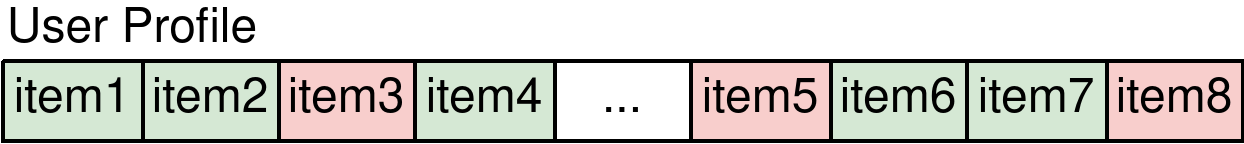
\includegraphics[scale=0.2]{pre-filtering1}
\end{figure}
\end{frame}
\begin{frame}
  \frametitle{Pre-filtering}
\begin{figure}
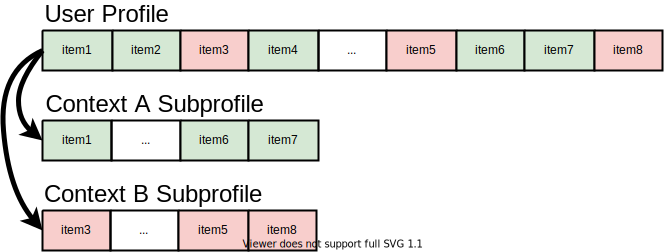
\includegraphics[scale=0.2]{pre-filtering2}
\end{figure}
\end{frame}
\begin{frame}
  \frametitle{Pre-filtering}
\begin{figure}
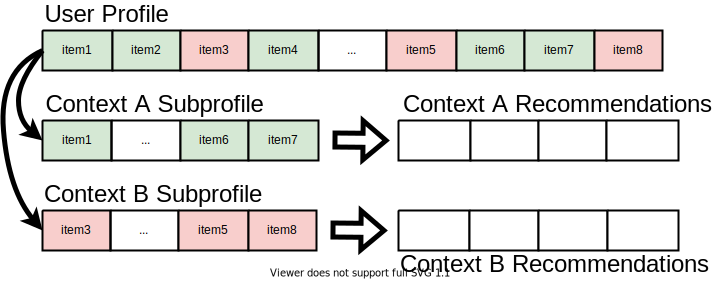
\includegraphics[scale=0.2]{pre-filtering3}
\end{figure}
\end{frame}
\begin{frame}
  \frametitle{Pre-filtering}
  \begin{itemize}
  \item get user's history
  \item filter only items relevant to current context
  \item recommend to user's sub-profile, not whole user
  \end{itemize}
\end{frame}
\begin{frame}
  \frametitle{Pre-filtering Problems}
  \begin{itemize}
  \item users' history should be very long
  \item and the more contexts you have, the longer
  \end{itemize}
\end{frame}
\begin{frame}
  \frametitle{Post-filtering}
\begin{figure}
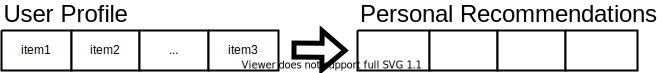
\includegraphics[scale=0.2]{post-filtering1}
\end{figure}
\end{frame}
\begin{frame}
  \frametitle{Post-filtering}
\begin{figure}
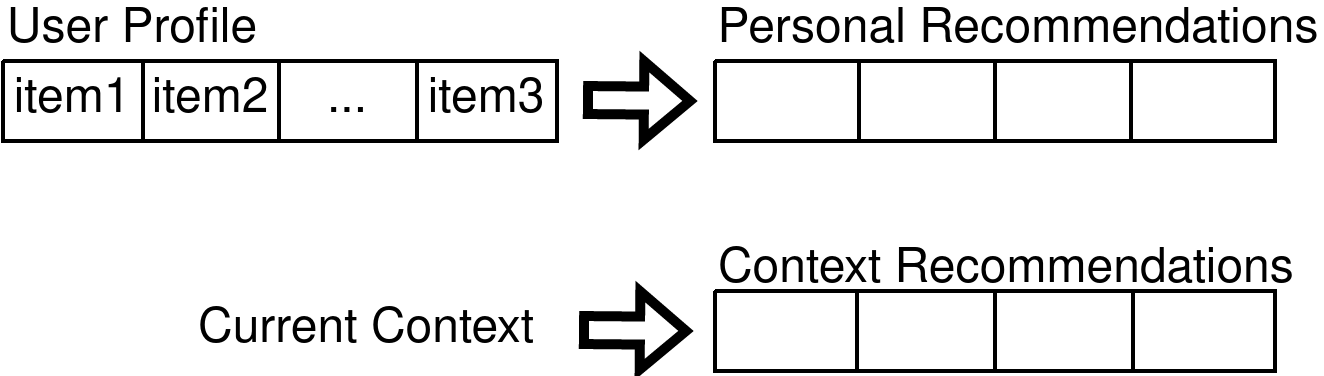
\includegraphics[scale=0.2]{post-filtering2}
\end{figure}
\end{frame}
\begin{frame}
  \frametitle{Post-filtering}
\begin{figure}
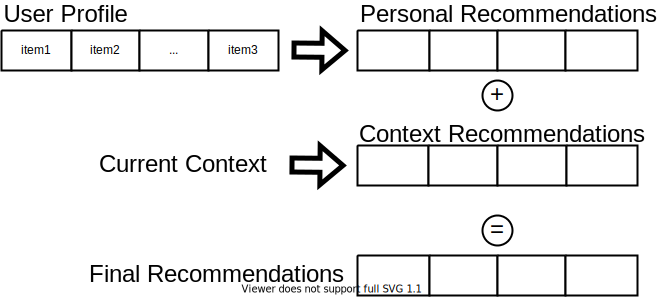
\includegraphics[scale=0.2]{post-filtering3}
\end{figure}
\end{frame}
\begin{frame}
  \frametitle{Post-filtering}
  \begin{itemize}
  \item get personal recommendations for a user
  \item get recommendations for current context
  \item combine personal and context recommendation
  \end{itemize}
\end{frame}
\begin{frame}
  \frametitle{Post-filtering}
  \begin{itemize}
  \item can work for shorter user histories
  \item you should have noticeable context trends
  \item or balancing between personal and context recs can be hard
  \end{itemize}
\end{frame}
\begin{frame}
  \frametitle{Context-aware Models: Training}
  \begin{figure}
  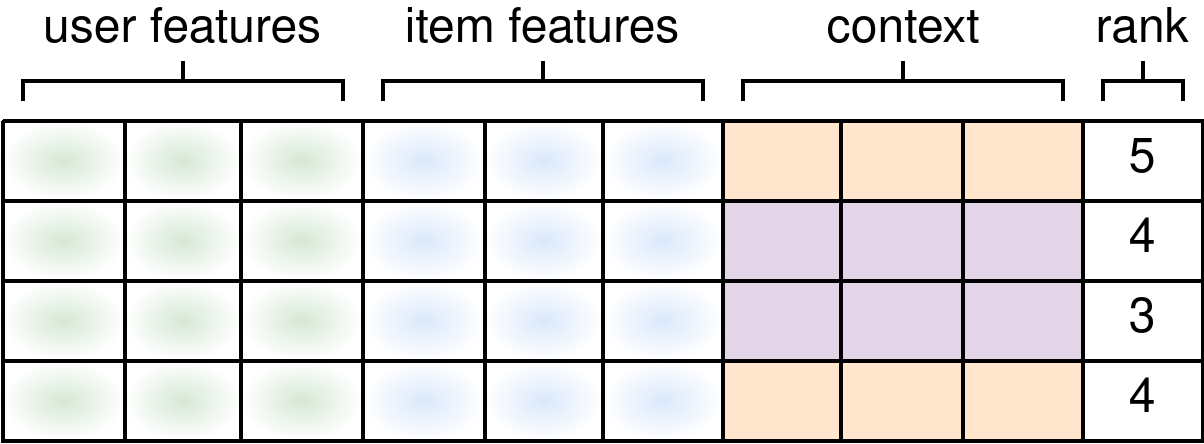
\includegraphics[scale=0.25]{context-aware-1}
  \end{figure}
\end{frame}
\begin{frame}
  \frametitle{Training: Item-Context is New Item!}
  \begin{figure}
  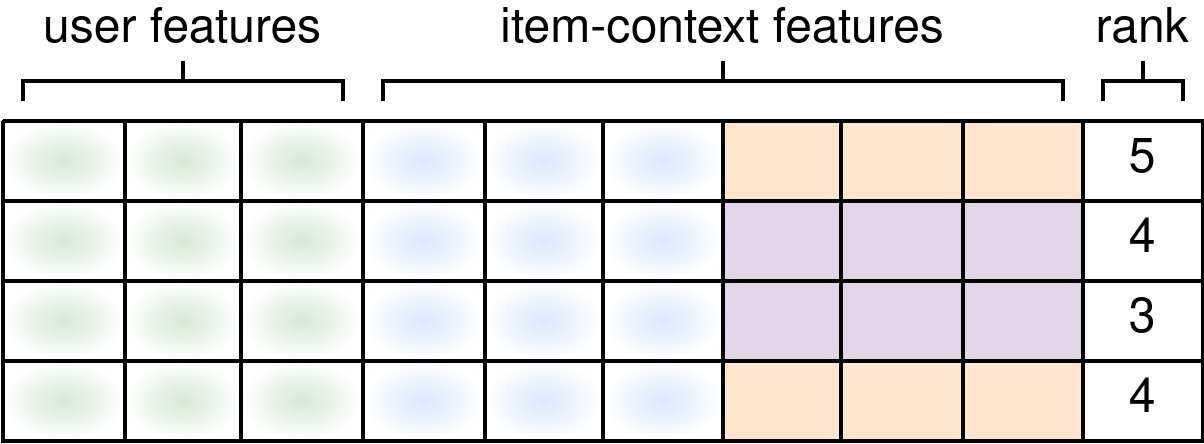
\includegraphics[scale=0.25]{context-aware-2}
  \end{figure}
\end{frame}
\begin{frame}
  \frametitle{Serving: Different Models for Each Context}
  \begin{figure}
  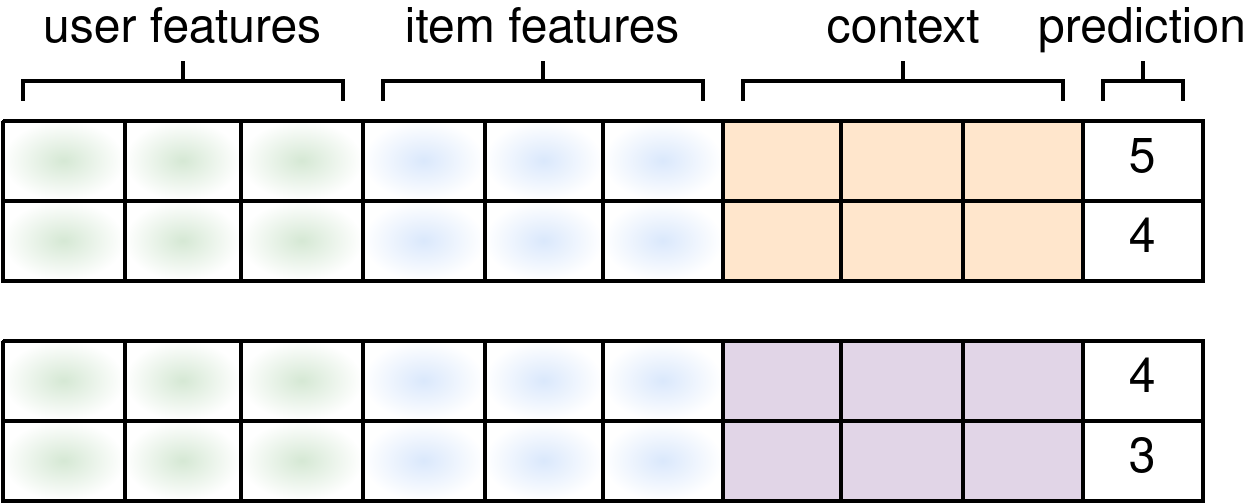
\includegraphics[scale=0.25]{context-aware-3}
  \end{figure}
\end{frame}
\begin{frame}
  \frametitle{Context-aware Models}
  \begin{itemize}
  \item training with classical models
  \item serving with separate model artifacts
  \item no problems from pre- or post-filtering
  \end{itemize}
\end{frame}
\begin{frame}
  \frametitle{Tucker Decomposition}
$$R_{uic}=\sum\limits_{j_u=1}^{r_U}\sum\limits_{j_i=1}^{r_I}\sum\limits_{j_c=1}^{r_C}X_{u,j_u}Y_{i,j_i}Z_{c,j_c}\Sigma_{j_u,j_i,j_c}$$
  
  where

  $R_{uic}$ --- rating dependant on user, item, and context

  $U,I,C$ --- numbers of users, items, and contexts
  
  $X_{u,j_u},Y_{i,j_i},Z_{c,j_c}$ --- matrices of (latent) user-factors, item-factors, and context-factors

  $r_U\ll U,r_I\ll I,r_C<C$ --- numbers of user-factors, item-factors, and context-factors

  $\Sigma_{j_u,j_i,j_c}$ --- a core tensor of $R_{uic}$, analogous to the matrix of singular values
\end{frame}
\begin{frame}
  \frametitle{Tucker Decomposition}
  \begin{figure}
  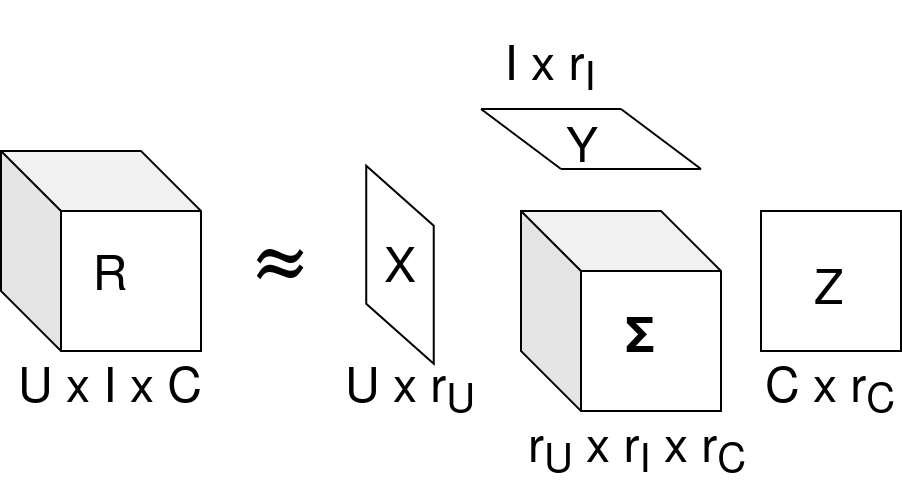
\includegraphics[scale=0.3]{tucker}
  \end{figure}
\end{frame}
\begin{frame}
  \begin{figure}
  \includegraphics[scale=0.45]{SVD}
  \end{figure}
\end{frame}
\begin{frame}
  \frametitle{Context-aware Recommenders}
  \begin{itemize}
  \item old models: pre-filtering and post-filtering
  \item new models: including context into the model
  \item particular case: Tucker decomposition
  \end{itemize}
\end{frame}
\section{Factorisation Machines}
\begin{frame}
  \frametitle{Factorisation Machines}
  \begin{itemize}
  \item invented by Steffen Rendle in 2010
  \item won several Kaggle competitions
  \item were a goto method for ranking step in RS in 2010s
  \item inspired some contemporary DL architectures
  \end{itemize}
\end{frame}
\begin{frame}
  \frametitle{Factorisation Machines: Data}
  \begin{figure}
    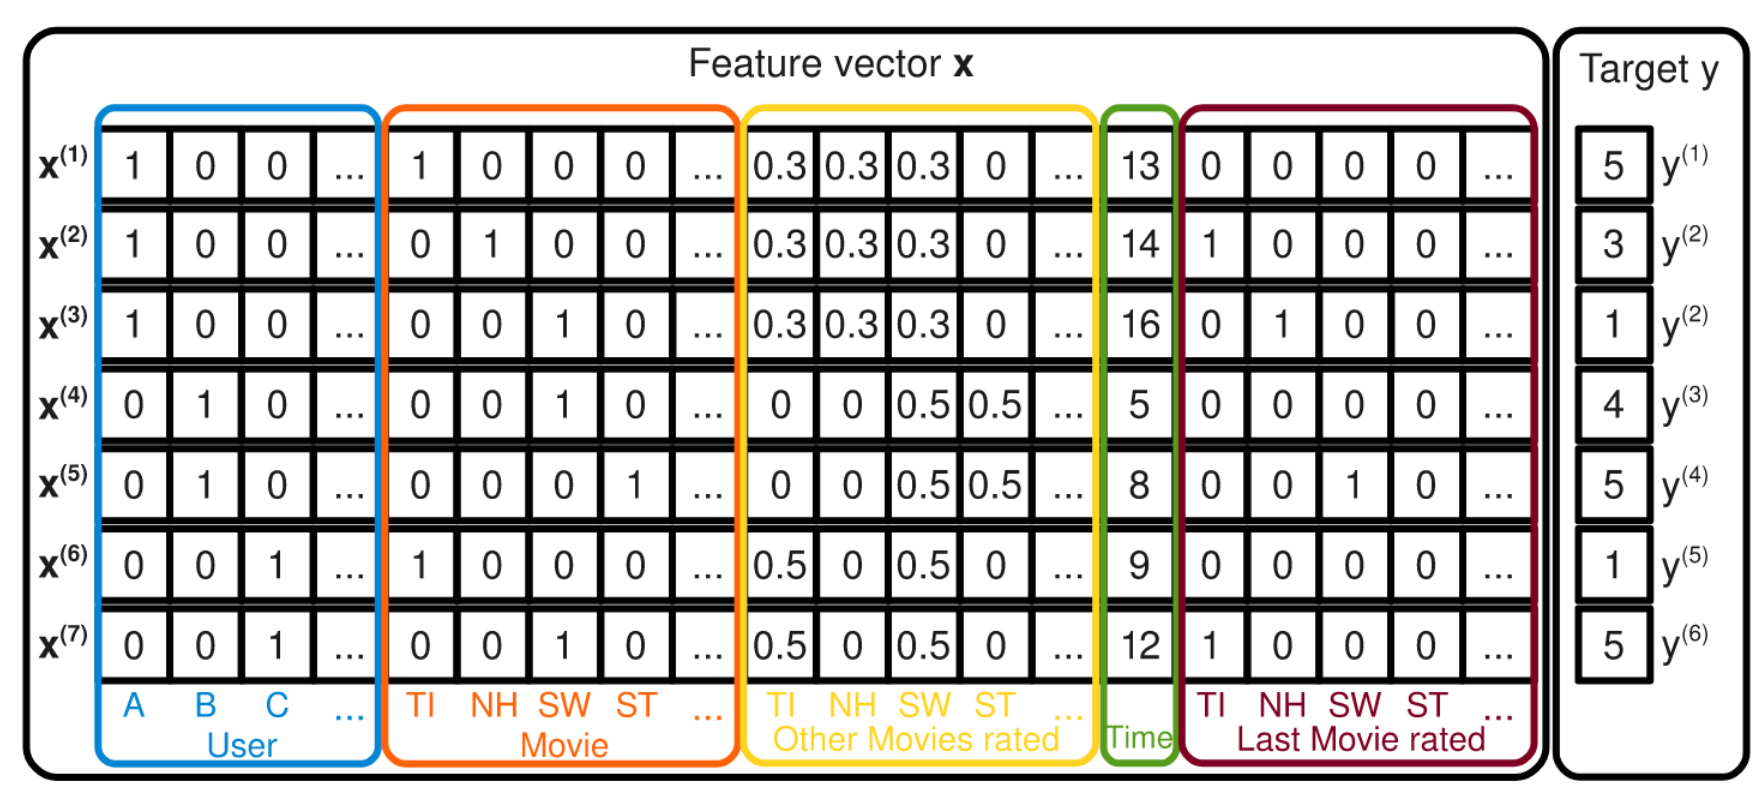
\includegraphics[scale=0.17]{fm}
  \end{figure}
  (source: DOI: 10.1109/ICDM.2010.127)
\end{frame}
\begin{frame}
  \frametitle{Factorisation Machines: Data}
  \begin{itemize}
  \item user ID and item ID are categorical features
  \item all features are treated equally
  \item can work for other ranking scenarios as well
  \end{itemize}
\end{frame}
\begin{frame}
  \frametitle{Factorisation Machines: Model}
  \begin{exampleblock}  {}$$r\left(x\right)=\omega_0+\sum\limits_{i=1}^n\omega_ix_i+\sum\limits_{i=1}^n\sum\limits_{j=1}^n\omega_{ij}x_ix_j$$
  \end{exampleblock}
  where
  \begin{itemize}
  \item $x$ --- features (one-hot-encoded item ID and user ID included)
  \item $n$ --- a dimension of $x$ (total number of features)
  \item $r\left(x\right)$ --- predicted rating of item for a user
  \item $\omega_0$ --- global bias
  \item $\omega_i$ --- feature biases (like item's popularity)
  \item $\omega_{ij}$ --- Hessian matrix
  \end{itemize}
\end{frame}
\begin{frame}
  \frametitle{Factorisation Machines: More Expressive}
  \begin{exampleblock}  {}$$r\left(x\right)=\omega_0+\sum\limits_{i=1}^n\omega_ix_i+\sum\limits_{i=1}^n\sum\limits_{j=1}^n\omega_{ij}x_ix_j$$
  \end{exampleblock}
  \begin{itemize}
  \item $n$ is extremely large (at least number of items plus number of users)
  \item $r\left(x\right)$ is predicted by a Maclaurin series up to the second term
  \item (this is similar to a basic matrix factorisation model)
  \item $\omega_{ij}$ includes not only bilinear (user-item)
  \item but also quadratic elements (item-item and user-user)
  \end{itemize}
\end{frame}
\begin{frame}
  \frametitle{Factorisation Machines: Main Idea}
  \begin{exampleblock}  {}$$r\left(x\right)=\omega_0+\sum\limits_{i=1}^n\omega_ix_i+\sum\limits_{i=1}^n\sum\limits_{j=1}^n\omega_{ij}x_ix_j$$
    $$\omega_{ij}=\left<v_i,v_j\right>$$
  \end{exampleblock}
  where
  \begin{itemize}
  \item $n$ is extremely large (at least number of items plus number of users)
  \item there are $n^2$ of $\omega_{ij}$ --- unreasonably many
  \item $\dim v_i=k\ll n$
  \item model has $kn + n + 1$ parameters
  \end{itemize}
\end{frame}
\begin{frame}
  \frametitle{Factorisation Machines: Usage}
  \begin{itemize}
  \item quadratic features can be a game changer (and can be encoded in a NN)
  \item \href{http://libfm.org/}{\texttt{LibFM}} --- package written by Rendle
  \item \href{https://pypi.org/project/turicreate}{\texttt{Turi Create}} --- a user-friendly implementation (now maintained by Apple)
  \item \href{https://github.com/ycjuan/libffm}{\texttt{LibFFM}} --- Field-Aware FM (can be used with Turi)
  \end{itemize}
\end{frame}
\begin{frame}
  \frametitle{LightFM is not a Factorisation Machine!}
  \begin{itemize}
  \item in LightFM one have only bilinear (user-item) terms
  \item FM must have quadratic (item-item and user-user) terms
  \item LightFM is a different model with only a distant similarity to FM
  \end{itemize}
\end{frame}
\begin{frame}
  \frametitle{Factorisation Machines: Conclusion}
  \begin{itemize}
  \item hard to beat technique for ranking tasks
  \item powerful but simple idea to implement yourself
  \item declined in popularity after the advent of DL
  \end{itemize}
\end{frame}
\section{Other Topics in Recommender Systems}
\begin{frame}
  \frametitle{Research topics we didn't talk about}
  \begin{itemize}
  \item reinforcement learning (counterfactual optimisation)
  \item learning metrics in hyperbolic geometry
  \item latent factors stability (PDE-related theorems)
  \item multi-step recommendations (conversational)
  \item theoretical upper bounds of quality metrics
  \item multi-criteria optimisation (e.g. precision vs diversity)
  \item privacy in recommender system
  \item fairness and bias in recommender systems
  \item managing recommender systems models in production
  \item correlation of mathematical and business metrics
  \item $\dots$
  \end{itemize}
\end{frame}
\end{document}
